\chapter{Experiments}

\section{Datasets}

Our RL agent is generating CNN architectures that are performing an image classification task on the CIFAR-10 and CIFAR-100 datasets.

CIFAR datasets are described in very deep detail in Chapter 3 of \cite{CIFAR}, especially details about its collection.

I would not go into details, just will note that CIFAR is a set of $32\times 32$ color images depicting real-world objects.

After training the RL algorithm on CIFAR10 it is heavily switched to use its knowledge on CIFAR100 to provide us with an idea about how this algorithm would handle knowledge transferring during the live experiment.

Key differences between CIFAR10 and CIFAR100 is denoted in table \ref{table:1}.

\begin{table}[h!]
\centering
\begin{tabular}{c c c c} 
 \hline
 Dataset & Size & Number of classes & Images in class \\ [0.5ex] 
 \hline
 CIFAR10 & 60000 & 10 & 6000 \\
 \hline
 CIFAR100 & 60000 & 100 grouped into 20 superclasses & 600 \\
 \hline \\ [0.5ex]
\end{tabular}
\caption{Comparison of CIFAR10 and CIFAR100 datasets}
\label{table:1}
\end{table}

Both in CIFAR10 classes are exclusive and do not assume instances overlapping - see \ref{fig:cifar10}. 

\begin{figure}[!htb]
  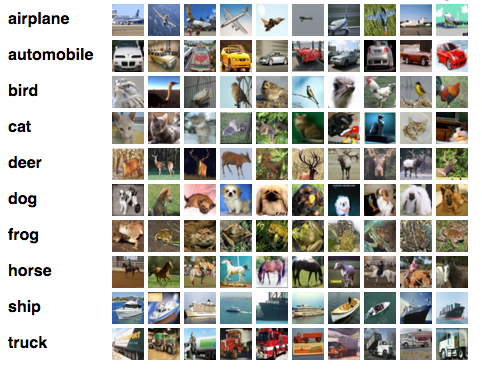
\includegraphics[width=\linewidth]{images/cifar10example.png}
  \caption{Classes of CIFAR10 including 10 random images from each \cite{CIFAR}}
  \label{fig:cifar10}
\end{figure}

We use CIFAR datasets as is, meaning that we also share the same train/test dataset split for evaluating generated CNN architectures. There are 50000 training images and 10000 test images in the dataset.

\section{Metrics}

Because of the nature of the problem that we are solving one metric would be in common for any approach described: it's a generated CNN accuracy. However, to see more details of the RL agent learning, we will use also additional metrics since we are handling two parallel experiments and since the Gaussian layer of a master CNN provides a distribution which gives us some additional knowledge.

\begin{table}[h!]
\centering
\begin{tabular}{c c c c} 
 \hline
 Algorithm & Loss Function & Additional metrics \\ [0.5ex] 
 \hline
 Classic CNN & Huber loss & 6000 \\
 \hline
 CNN with Gaussian Layer & MLE of variance & $\mu$ and $\sigma$ \\
 \hline \\ [0.5ex]
\end{tabular}
\caption{Additional metrics of RL algorithm}
\label{table:2}
\end{table}

\section{Environment and training}

Our models are implemented using Pytorch [\cite{NEURIPS2019_9015}] (master CNN) and Tensorflow [\cite{tensorflow2015-whitepaper}](slave CNN). There was no particular need to develop them using different frameworks, it's a historical issue.

RL agent was trained on the GPU resources provided by Google Colaboratory [\cite{colab}] service.

Each RL agent was trained for 80 epochs on the first dataset (CIFAR10) and then hard-switched to CIFAR100 (leaving weights of the backend CNN, but clearing other metadata).

First 10 epoch there were 9 random actions explored. This number decayed by 1 every 10 epochs until int finally will become 1 random action per 10 epochs.

RL agent was choosing 4 kernel size and filter sizes tuples from available sizes. Types of slave CNN hidden layers were predefined.

\begin{table}[h!]
\centering
\begin{tabular}{c c c c} 
 \hline
	Action type & Values available in experiment\\ [0.5ex] 
 \hline
	Filter size & 1, 3, 6, 9, 12, 24 \\
 \hline
	Filter size & 2, 4, 8, 16, 32, 64 \\
 \hline \\ [0.5ex]
\end{tabular}
\caption{Action space description}
\label{table:3}
\end{table} 

Each slave CNN was trained for 8 epochs.

\section{Results}

\begin{figure}[!htb]
  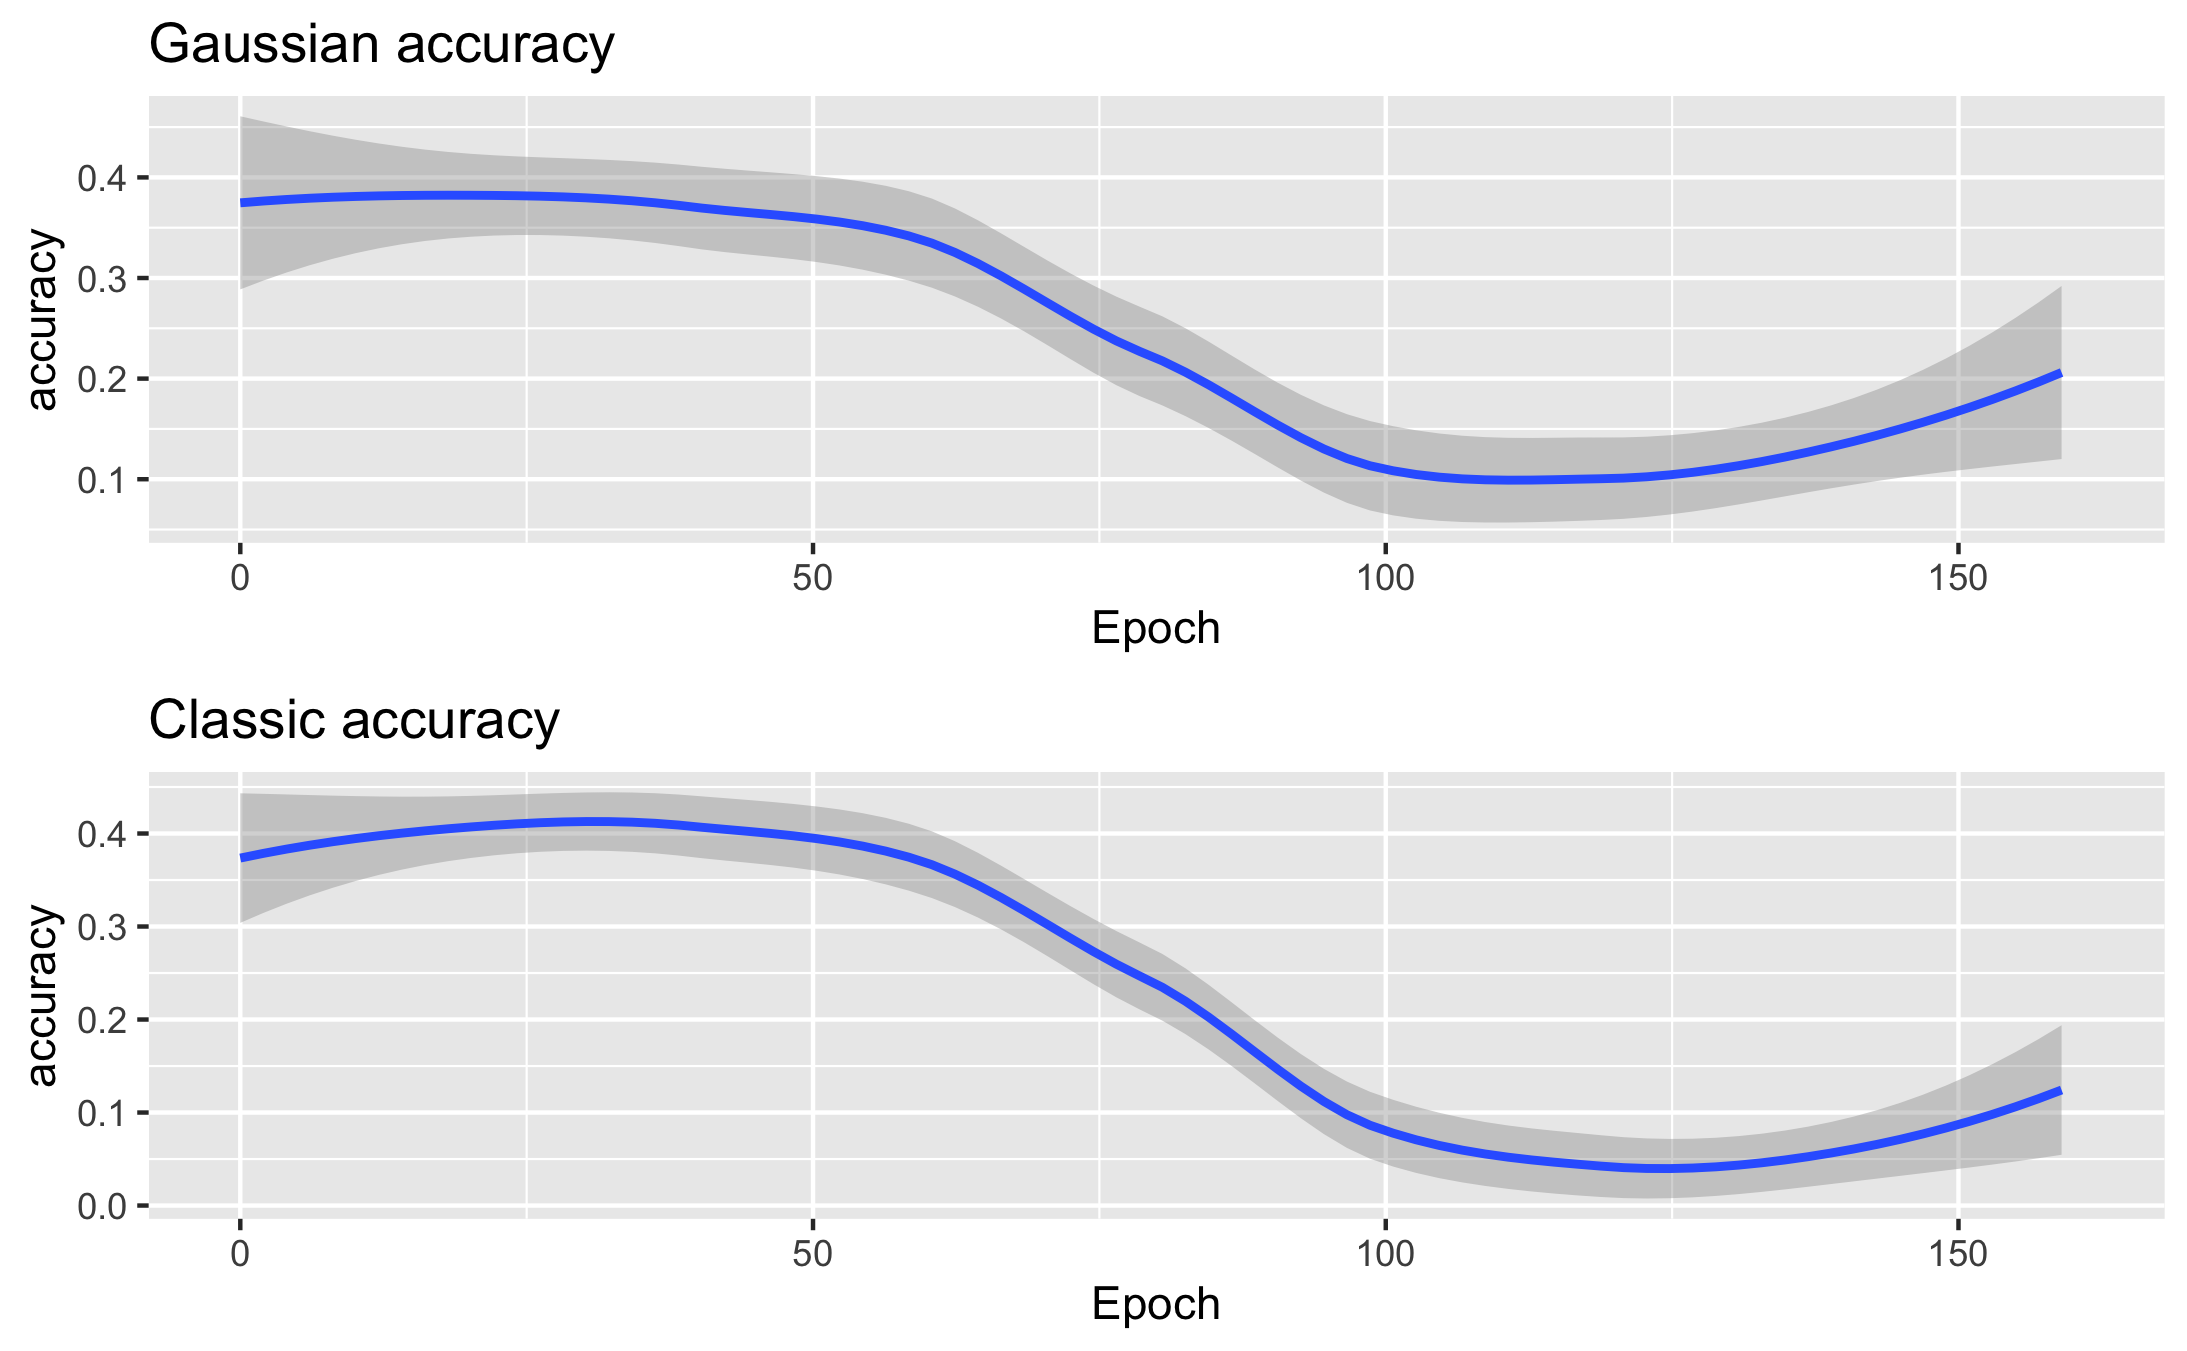
\includegraphics[width=\linewidth]{images/epsilon_greedy.png}
  \caption{Accuracy of slave CNN generated via epsilon-greedy approach}
  \label{fig:egreedy}
\end{figure}

\begin{figure}[!htb]
  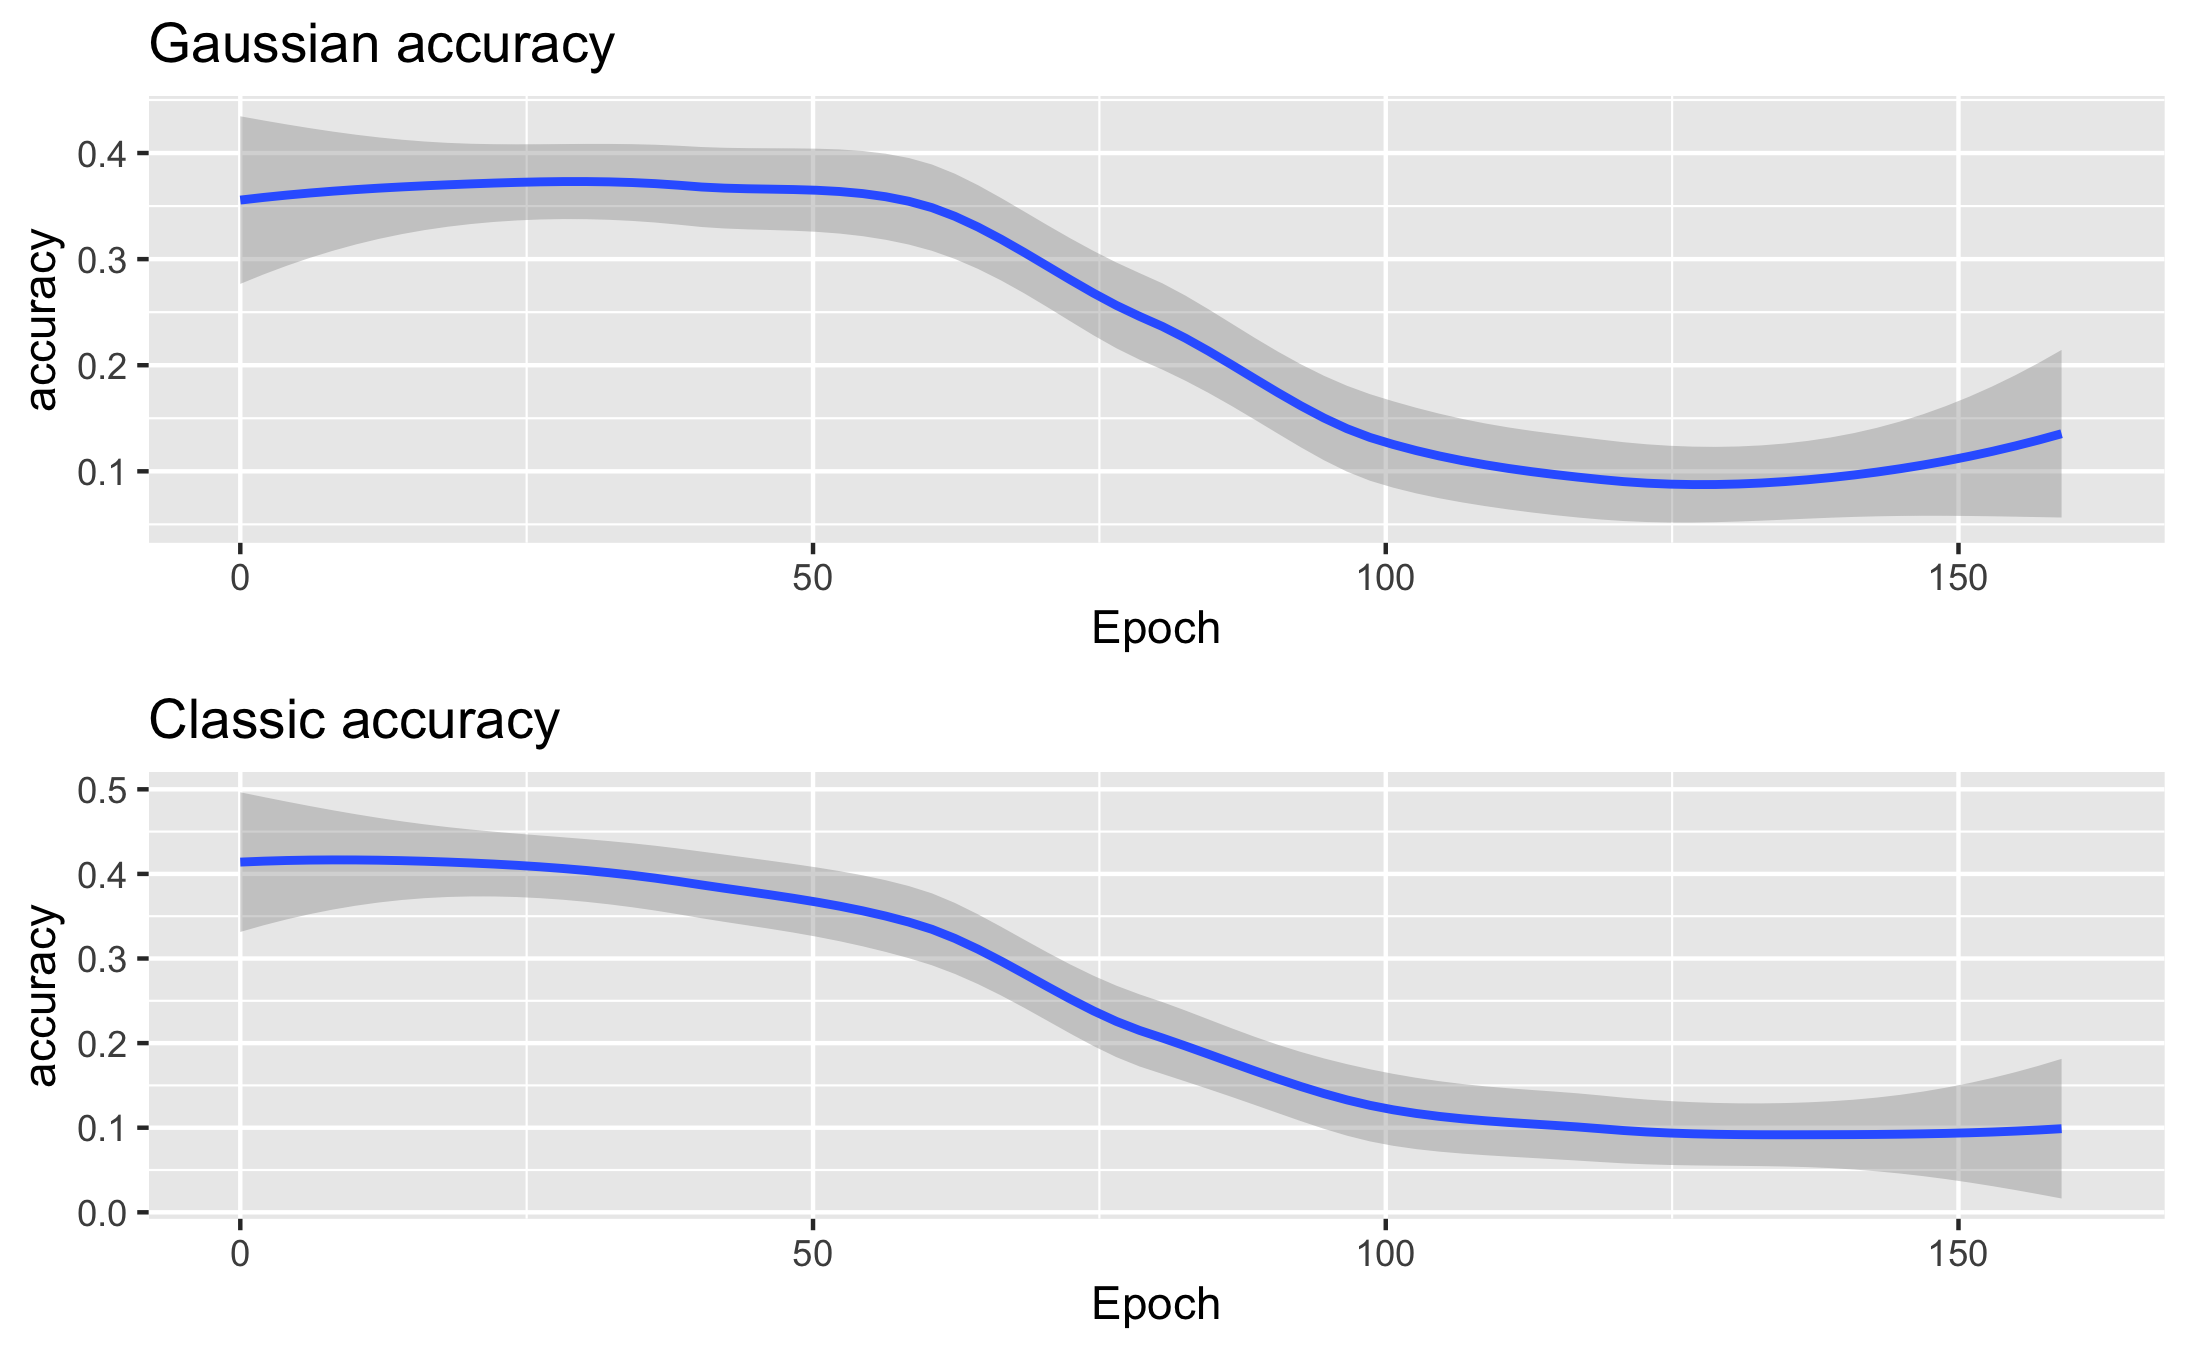
\includegraphics[width=\linewidth]{images/ucb.png}
  \caption{Accuracy of slave CNN generated via upper confidence bound approach}
  \label{fig:ucbs}
\end{figure}

Even though that chart looks similar to each other there are few things to note here:

\begin{itemize}
\item UCB does not provide any benefits to the algorithm in this configuration and environment setup
\item During numerous sets of experiments we've seen that Gaussian modification yields better CNN architectures while handling knowledge transfer problems.
\end{itemize}

Even though yielding 0.2 accuracies after 8 epochs of training on CIFAR100 is a good result, it is interesting to see how these agents was actually training. Since the goal of RL agent is the maximization of cumulative reward it would be beneficial to see how this reward was changing over time (see \ref{fig:totrewegreedy}).

\begin{figure}[!htb]
  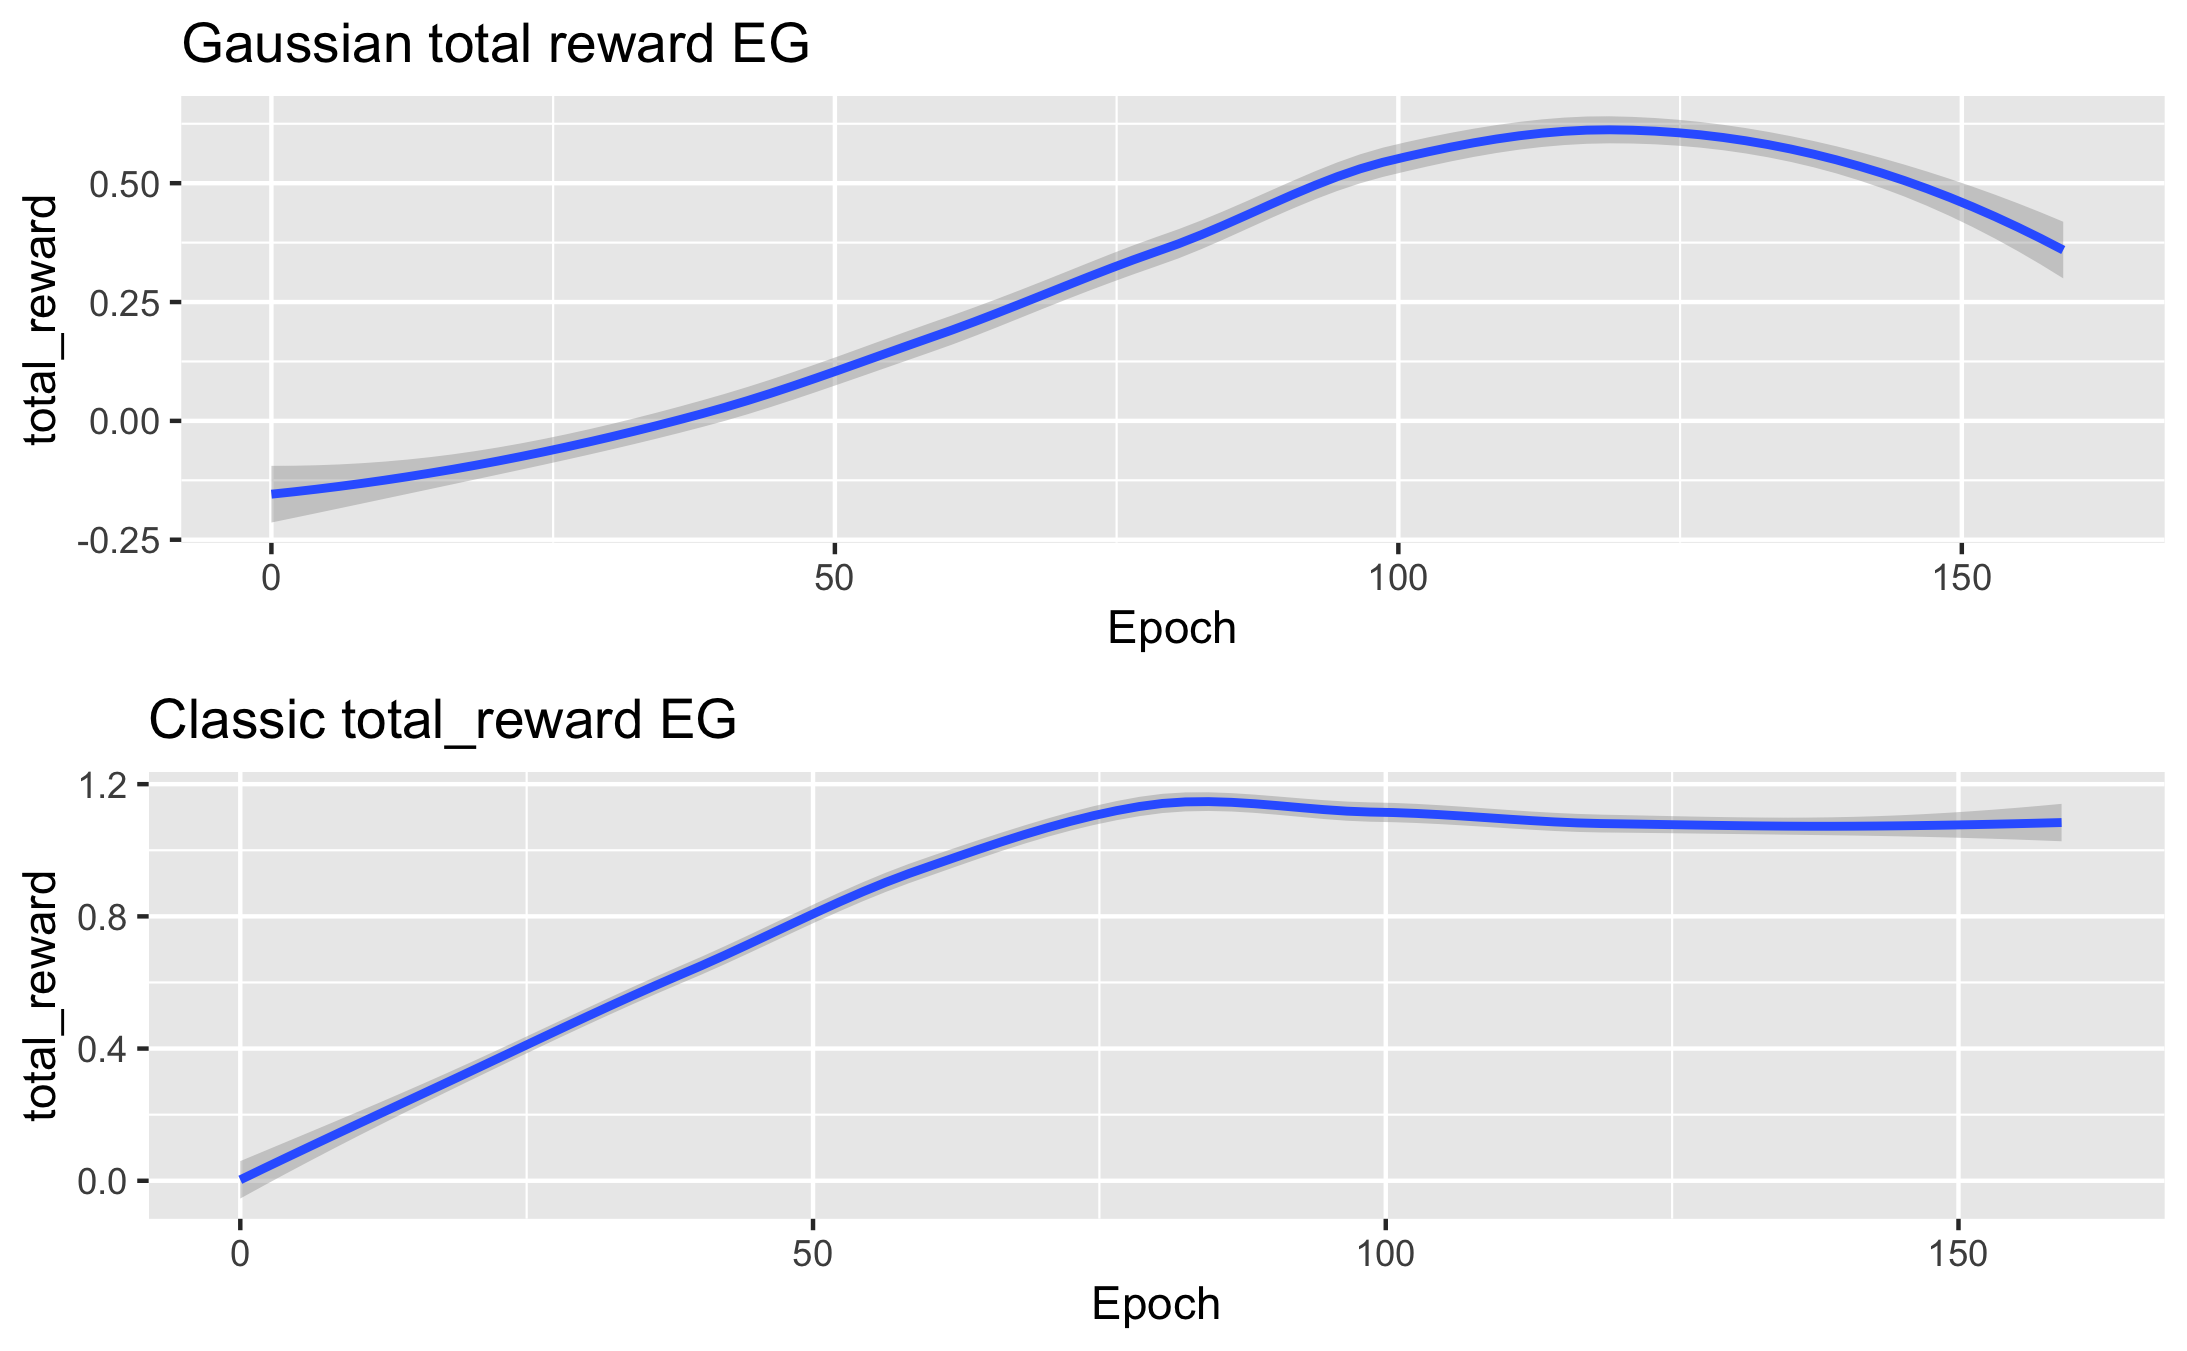
\includegraphics[width=\linewidth]{images/total_reward_epsilon_greedy.png}
  \caption{Total reward of both RL controllers compared}
  \label{fig:totrewegreedy}
\end{figure}

Since RL agent receives moving accuracy from the controller both of those lines will stop increasing after the dataset would changes. Obviously, results received on CIFAR100 would be much lower than on CIFAR10. That's why we should see those lines moving down after the dataset was changed if the RL algorithm is still training. This is the reason why the classic algorithm performed twice as low as Gaussian one after the dataset was hard-changed.

To estimate how the agent learns, we must see how it exploits it's knowledge (see \ref{fig:actionunique}). Blue lines indicate an action that was already generated or explored by the controller at some point in time before. It's interesting to see how both algorithms react to the change in their MDP state because of the database change.

\begin{figure}[!htb]
  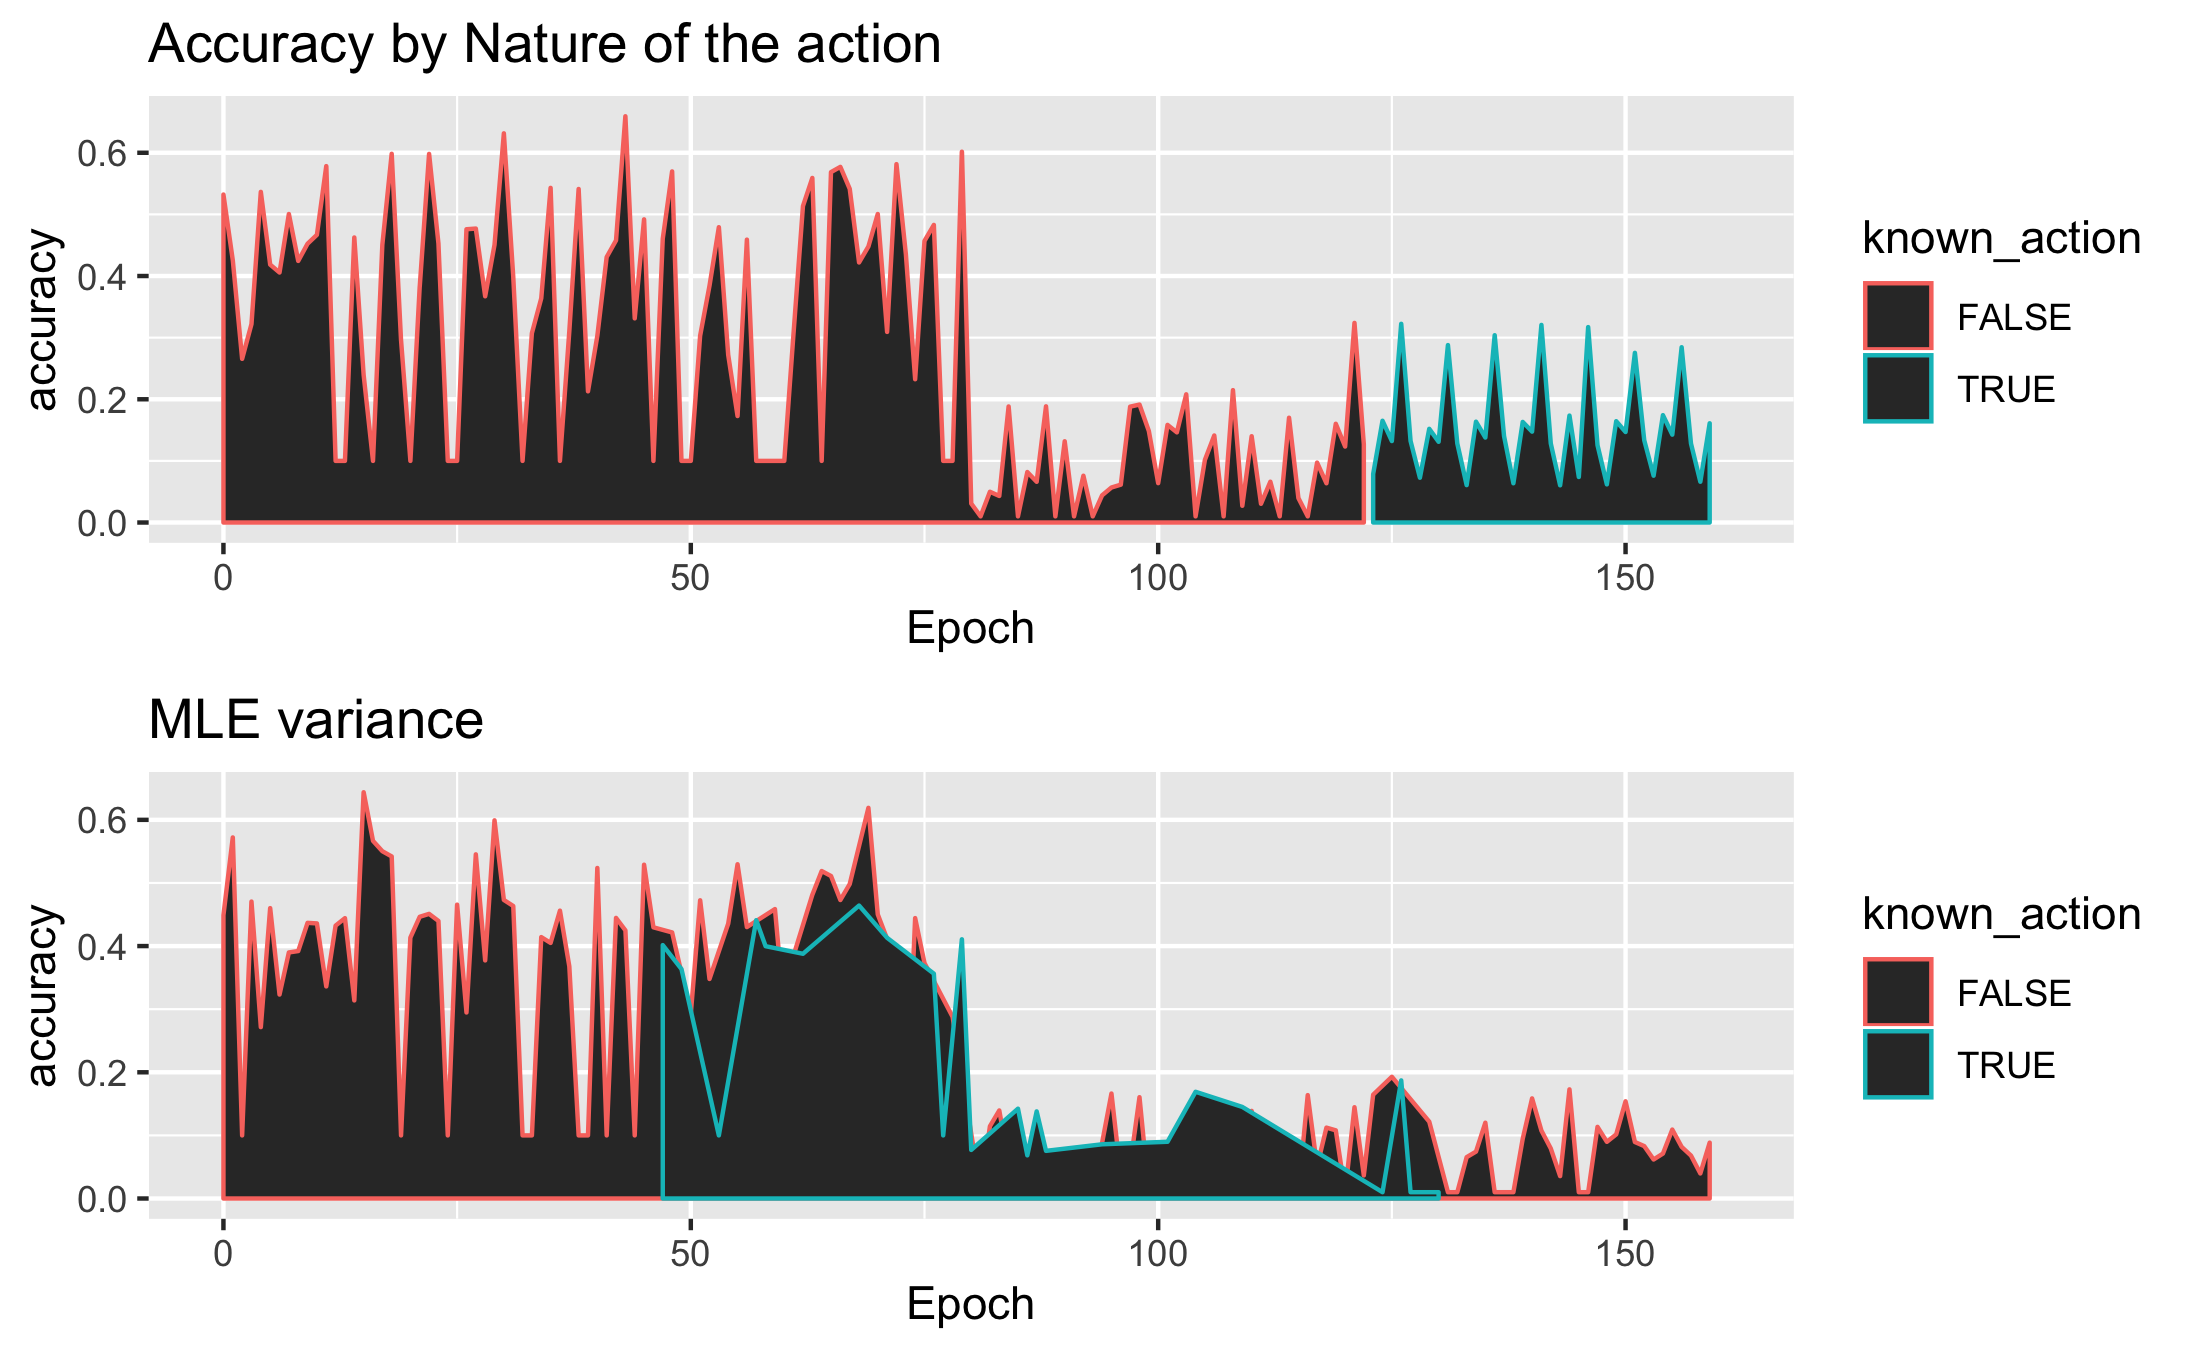
\includegraphics[width=\linewidth]{images/action_unique.png}
  \caption{Distribution of knowledge exploitation during the training}
  \label{fig:actionunique}
\end{figure}

Finally let's see how $\mu$ and $\sigma$ distribution changed during the period of training (see \ref{fig:musigma}).

\begin{figure}[!htb]
  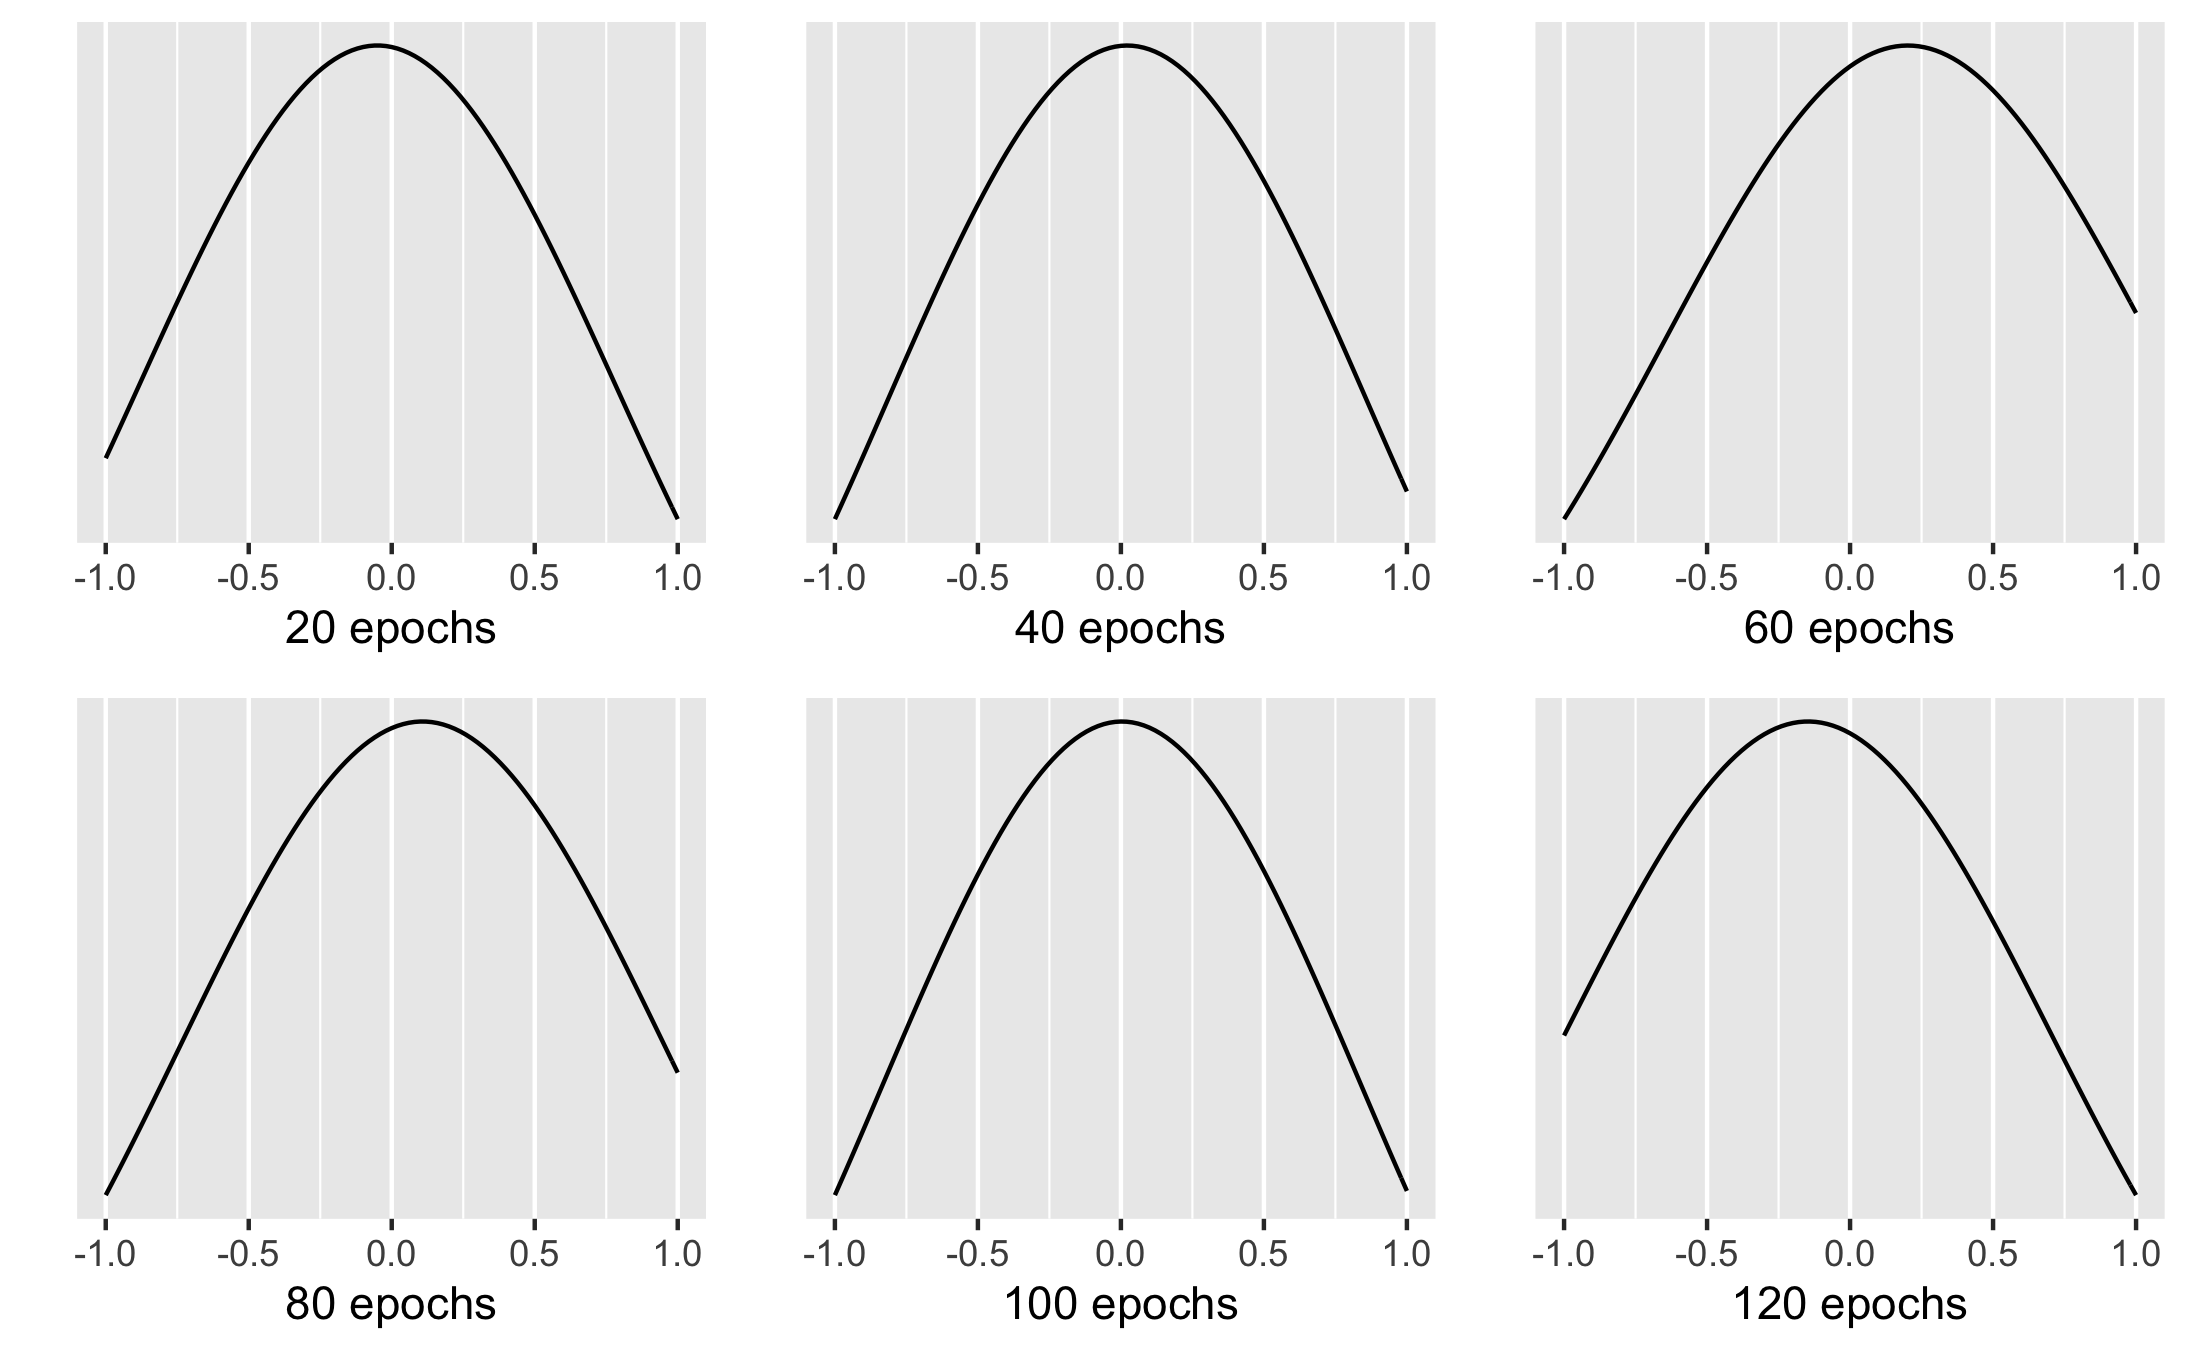
\includegraphics[width=\linewidth]{images/musigma.png}
  \caption{Gaussian distributions received on the last layer of CNN}
  \label{fig:musigma}
\end{figure}

Notice how the standard deviation of the distribution becomes bigger as the underlying CNN train and then reduces again when the dataset was updated. This would be more interesting to explore on a larger time scale, however, even on the 80-epoch experiment Gaussian approach shows it's strong ability to generate better architectures exploiting existing knowledge. It also seems to avoid a lot of overfitting problems.

\begin{table}[h!]
\centering
\begin{tabular}{c c c} 
 \hline
 Algorithm & CIFAR10 avg last 10 epoch & CIFAR100 avg last 10 epoch \\ [0.5ex] 
 \hline
 Gaussian epsilon-greedy & 0.3807 & 0.1588\\
 \hline
 Classic epsilon-greedy & 0.3308 & 0.0846 \\
 \hline
 Gaussian UCB & 0.3875 & 0.1078\\
 \hline
 Classic UCB & 0.3737 & 0.0799\\
 \hline \\ [0.5ex]
\end{tabular}
\caption{Accuracy achieved by slave CNN}
\label{table:5}
\end{table}

However, during this experiments some issues were found:

\begin{itemize}
\item{RL algorithms are not very stable and occasionally they can yield bad results as seen at \ref{fig:actionunique}}
\item{Training of those algorithms in a way proposed is resource-ineffective and in any other research should be done using NASbench \cite[see]{pmlr-v97-ying19a}}
\item{Even though gaussian distribution yields better results it hasn't prevented algorithm from overfitting at small action space}.
\end{itemize}
